% ============================================================
\chapter{O módulo \texttt{math}}
\label{cap:aula3}
% ============================================================

\begin{objetivos}
\begin{itemize}
  \item entender o que é um módulo e as formas de importá-lo;
  \item usar as constantes e funções do módulo \py{math}: piso, teto, raízes, exponencial, logaritmos,
        trigonométricas, fatorial e combinações;
  \item programar a raiz quadrada pelo \textbf{método babilônico} e comparar com \py{math.sqrt};
  \item usar \py{math} em aplicações: teorema de Pitágoras, lei dos cossenos, teste de primalidade e o
        método da bissecção.
\end{itemize}
\end{objetivos}

\begin{roteiro}
0--10 min & Módulos: \py{import}, \py{as}, \py{from ... import}; ajuda com \py{help} e \py{dir}.\\
10--30 min & Funções do \py{math}: piso/teto, raízes, exp/log, trigonometria, funções inteiras.\\
30--40 min & Aplicação: Pitágoras e lei dos cossenos.\\
40--60 min & Atividade principal: raiz quadrada pelo método babilônico.\\
60--75 min & Teste de primalidade e método da bissecção.\\
75--90 min & Exercícios.\\
\end{roteiro}

% ------------------------------------------------------------
\section{Módulos e importação}
% ------------------------------------------------------------

O Python ``puro'' só sabe fazer as operações básicas. Funções como raiz quadrada, seno ou logaritmo estão em
\textbf{módulos} (bibliotecas), que precisam ser \emph{importados}. O módulo \py{math} faz parte da instalação
padrão do Python e contém as funções matemáticas elementares para números reais (\py{int} e \py{float}).

Há três formas usuais de importar:

\begin{entrada}
import math                  # 1) importa o módulo inteiro
print(math.sqrt(2), math.pi)

import math as m             # 2) importa com um apelido
print(m.sqrt(2))

from math import sqrt, pi    # 3) importa só alguns nomes
print(sqrt(2) * pi)
\end{entrada}
\begin{saida}
1.4142135623730951 3.141592653589793
1.4142135623730951
4.442882938158366
\end{saida}

\begin{itemize}
  \item Na forma 1, os nomes são usados com o prefixo \py{math.} (\emph{math ponto}).
  \item Na forma 2, o prefixo é o apelido (\py{m.}). É a forma usada com NumPy (\py{np}) e SymPy (\py{sp}).
  \item Na forma 3, os nomes importados são usados sem prefixo.
\end{itemize}

\begin{atencao}
Existe também \py{from math import *}, que importa \emph{todos} os nomes. Evite: fica difícil saber de onde veio
cada função e, mais adiante, o \py{sin} do \py{math}, o do NumPy e o do SymPy vão ``brigar'' entre si.
\end{atencao}

\begin{dica}
Para ver todas as funções do módulo, execute \py{dir(math)}. Para ler a ajuda de uma função,
\py{help(math.log)}. No Jupyter, digite \py{math.} e aperte \textbf{Tab} para ver a lista de opções.
\end{dica}

\begin{entrada}
help(math.log)
\end{entrada}
\begin{saida}
Help on built-in function log in module math:

log(...)
    log(x, [base=math.e])
    Return the logarithm of x to the given base.

    If the base is not specified, returns the natural logarithm (base e) of x.

\end{saida}

% ------------------------------------------------------------
\section{Constantes e funções do módulo \texttt{math}}
% ------------------------------------------------------------

\begin{center}\small
\renewcommand{\arraystretch}{1.15}
\begin{tabular}{@{}lll@{}}
\toprule
\textbf{Matemática} & \textbf{Python} & \textbf{Observação}\\
\midrule
$\pi$, $e$ & \py{math.pi}, \py{math.e} & aproximações \py{float}\\
$\infty$ & \py{math.inf} & ``infinito'' (\py{float})\\
$\lfloor x\rfloor$, $\lceil x\rceil$ & \py{math.floor(x)}, \py{math.ceil(x)} & piso e teto (devolvem \py{int})\\
$|x|$ & \py{abs(x)} ou \py{math.fabs(x)} & \py{abs} não precisa do \py{math}\\
$\sqrt{x}$ & \py{math.sqrt(x)} & $x\ge 0$\\
$\lfloor\sqrt{n}\rfloor$ & \py{math.isqrt(n)} & raiz inteira\\
$\sqrt[3]{x}$ & \py{math.cbrt(x)} & aceita $x<0$\\
$x^y$ & \py{x**y} ou \py{math.pow(x, y)} & \\
$e^x$ & \py{math.exp(x)} & \\
$\ln x$ & \py{math.log(x)} & logaritmo natural\\
$\log_b x$ & \py{math.log(x, b)} & \\
$\log_{10} x$, $\log_2 x$ & \py{math.log10(x)}, \py{math.log2(x)} & \\
$\sin x$, $\cos x$, $\tan x$ & \py{math.sin(x)}, \py{math.cos(x)}, \py{math.tan(x)} & em \textbf{radianos}\\
$\arcsin x$, $\arccos x$, $\arctan x$ & \py{math.asin(x)}, \py{math.acos(x)},\\ & \py{math.atan(x)} & em radianos\\
graus $\leftrightarrow$ radianos & \py{math.radians(g)}, \py{math.degrees(r)} & \\
$\sinh x$, $\cosh x$, $\tanh x$ & \py{math.sinh(x)}, \py{math.cosh(x)}, \py{math.tanh(x)} & \\
$n!$ & \py{math.factorial(n)} & $n$ inteiro $\ge 0$\\
$\binom{n}{k}$, $\frac{n!}{(n-k)!}$ & \py{math.comb(n, k)}, \py{math.perm(n, k)} & combinações e arranjos\\
$\mathrm{mdc}$, $\mathrm{mmc}$ & \py{math.gcd(a, b)}, \py{math.lcm(a, b)} & aceitam vários argumentos\\
$\sqrt{x^2+y^2}$ & \py{math.hypot(x, y)} & hipotenusa\\
$a\approx b$ & \py{math.isclose(a, b)} & compara \py{float}s\\
\bottomrule
\end{tabular}
\end{center}

\begin{maxima}
No Maxima as funções estão sempre disponíveis: \texttt{sqrt(2)}, \texttt{log(x)}, \texttt{sin(x)},
\texttt{\%pi}, \texttt{\%e}. Além disso, o Maxima devolve \texttt{sqrt(2)} de forma \emph{exata}, enquanto o
\py{math.sqrt(2)} devolve um número aproximado. O comportamento ``exato'' do Maxima será obtido com o SymPy
(Aulas 7 a 10). Note também que no Maxima \texttt{log} é o logaritmo natural, assim como no Python.
\end{maxima}

\subsection{Piso, teto e arredondamentos}

O \textbf{piso} $\lfloor x\rfloor$ é o maior inteiro menor ou igual a $x$, e o \textbf{teto} $\lceil x\rceil$ é o menor
inteiro maior ou igual a $x$:
\[
\lfloor x\rfloor = \max\{m\in\ZZ : m\le x\},\qquad \lceil x\rceil=\min\{n\in\ZZ : n\ge x\}.
\]

\begin{figure}[ht]
\centering
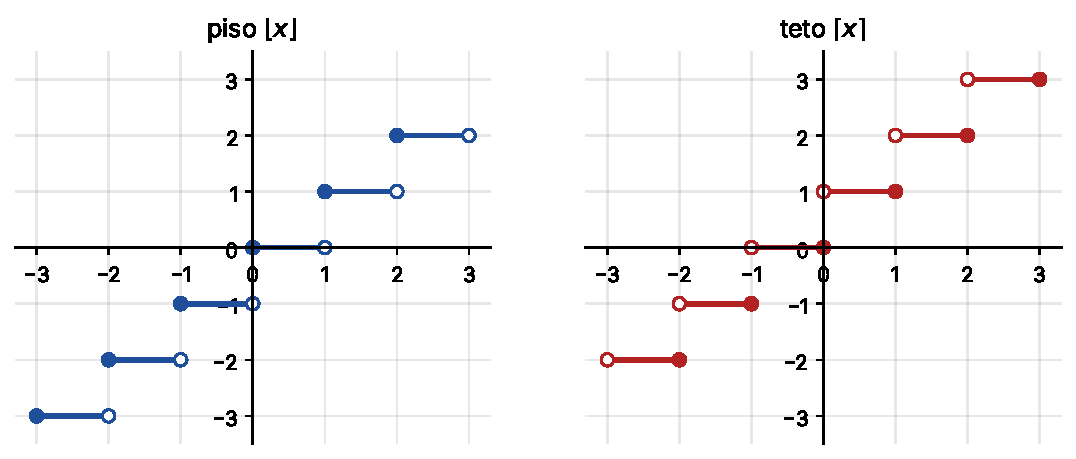
\includegraphics[width=0.85\linewidth]{aula03-piso-teto}
\caption{Gráficos das funções piso e teto. A bolinha cheia indica o valor da função no ponto de salto.}
\end{figure}

\begin{entrada}
for x in [2.1, 2.7, -2.1, -2.7, 3.0]:
    print(f"x = {x:5}  piso = {math.floor(x):3}  teto = {math.ceil(x):3}"
          f"  trunc = {math.trunc(x):3}  round = {round(x):3}")
\end{entrada}
\begin{saida}
x =   2.1  piso =   2  teto =   3  trunc =   2  round =   2
x =   2.7  piso =   2  teto =   3  trunc =   2  round =   3
x =  -2.1  piso =  -3  teto =  -2  trunc =  -2  round =  -2
x =  -2.7  piso =  -3  teto =  -2  trunc =  -2  round =  -3
x =   3.0  piso =   3  teto =   3  trunc =   3  round =   3
\end{saida}

Observe que para números negativos o piso e o \py{trunc} (que apenas descarta a parte decimal, como \py{int()})
são diferentes.

\begin{observacao}
O \py{round} do Python usa o ``arredondamento do banqueiro'': quando o número está exatamente no meio, arredonda
para o \emph{par} mais próximo. Assim \py{round(2.5)} dá \py{2} e \py{round(3.5)} dá \py{4}.
\end{observacao}

\subsection{Raízes, exponenciais e logaritmos}

\begin{entrada}
print(math.sqrt(16), math.sqrt(2), math.cbrt(-8))
print(math.isqrt(50))                 # maior inteiro k com k*k <= 50
print(math.exp(1), math.e)
print(math.log(math.e), math.log(100, 10), math.log10(0.001), math.log2(1024))
\end{entrada}
\begin{saida}
4.0 1.4142135623730951 -2.0
7
2.718281828459045 2.718281828459045
1.0 2.0 -3.0 10.0
\end{saida}

Fora do domínio, as funções do \py{math} geram erro:

% erro
\begin{entrada}
math.sqrt(-4)
\end{entrada}
\begin{saida}
ValueError: math domain error
\end{saida}

Para raízes de números negativos (resultados complexos) existe o módulo \py{cmath}, com as mesmas funções:

\begin{entrada}
import cmath
print(cmath.sqrt(-4), (-4)**0.5)
\end{entrada}
\begin{saida}
2j (1.2246467991473532e-16+2j)
\end{saida}

\paragraph{Exemplo: juros compostos.} Um capital aplicado a uma taxa de 1\% ao mês dobra quando $(1{,}01)^n=2$,
isto é, $n=\dfrac{\ln 2}{\ln 1{,}01}$.

\begin{entrada}
n = math.log(2) / math.log(1.01)
print(f"n = {n:.2f} meses, ou seja, {math.ceil(n)} meses")
\end{entrada}
\begin{saida}
n = 69.66 meses, ou seja, 70 meses
\end{saida}

\subsection{Trigonometria}

As funções trigonométricas usam o ângulo em \textbf{radianos}. Para trabalhar em graus, converta com
\py{math.radians}.

\begin{entrada}
print(math.sin(math.pi/2), math.cos(math.pi))
print(math.sin(30))                     # 30 RADIANOS, não graus!
print(math.sin(math.radians(30)))       # sen(30°)
print(math.degrees(math.atan(1)))       # arctan(1) em graus
print(math.sin(math.pi))                # deveria ser 0...
\end{entrada}
\begin{saida}
1.0 -1.0
-0.9880316240928618
0.49999999999999994
45.0
1.2246467991473532e-16
\end{saida}

O último valor, $1{,}22\times10^{-16}$, é ``zero com erro de arredondamento'': \py{math.pi} é apenas uma
aproximação de $\pi$. Valores muito pequenos como esse devem ser lidos como zero.

\begin{entrada}
print(" graus    sen      cos      tg")
for g in [0, 30, 45, 60]:
    r = math.radians(g)
    print(f"{g:5d} {math.sin(r):8.4f} {math.cos(r):8.4f} {math.tan(r):8.4f}")
\end{entrada}
\begin{saida}
 graus    sen      cos      tg
    0   0.0000   1.0000   0.0000
   30   0.5000   0.8660   0.5774
   45   0.7071   0.7071   1.0000
   60   0.8660   0.5000   1.7321
\end{saida}

\subsection{Funções para inteiros}

\begin{entrada}
print(math.factorial(10), math.factorial(25))
print(math.comb(60, 6))           # jogos possíveis na Mega-Sena
print(math.perm(5, 2))            # arranjos de 5 tomados 2 a 2
print(math.gcd(252, 198), math.lcm(4, 6, 10))
\end{entrada}
\begin{saida}
3628800 15511210043330985984000000
50063860
20
18 60
\end{saida}

% ------------------------------------------------------------
\section{Aplicações em geometria}
% ------------------------------------------------------------

\paragraph{Teorema de Pitágoras.} Em um triângulo retângulo de catetos $a$, $b$ e hipotenusa $c$, vale
$c^2=a^2+b^2$. O exemplo abaixo é o do livro da SBM.

% entradas: 10 | 11
\begin{entrada}
from math import sqrt
a = float(input("Digite o primeiro cateto: "))
b = float(input("Digite o segundo cateto: "))
c = sqrt(a**2 + b**2)          # ou math.hypot(a, b)
print("Hipotenusa:", c)
\end{entrada}
\begin{saida}
Digite o primeiro cateto: 10
Digite o segundo cateto: 11
Hipotenusa: 14.866068747318506
\end{saida}

\paragraph{Lei dos cossenos e fórmula de Herão.} Para um triângulo de lados $a,b,c$, o ângulo $\gamma$ oposto a
$c$ satisfaz $c^2=a^2+b^2-2ab\cos\gamma$, e a área é
$A=\sqrt{s(s-a)(s-b)(s-c)}$, com $s=\frac{a+b+c}{2}$.

\begin{entrada}
def angulos(a, b, c):
    """Ângulos (em graus) opostos aos lados a, b, c."""
    alfa = math.degrees(math.acos((b**2 + c**2 - a**2) / (2*b*c)))
    beta = math.degrees(math.acos((a**2 + c**2 - b**2) / (2*a*c)))
    gama = 180 - alfa - beta
    return alfa, beta, gama

def area_herao(a, b, c):
    s = (a + b + c) / 2
    return math.sqrt(s*(s - a)*(s - b)*(s - c))

print(angulos(3, 4, 5))
print(area_herao(3, 4, 5), area_herao(5, 5, 5))
\end{entrada}
\begin{saida}
(36.86989764584401, 53.13010235415599, 90.0)
6.0 10.825317547305483
\end{saida}

% ------------------------------------------------------------
\section{Atividade: a raiz quadrada pelo método babilônico}
% ------------------------------------------------------------

Como uma calculadora (ou o \py{math.sqrt}) calcula $\sqrt{2}$? Uma ideia muito antiga, atribuída aos
babilônios e descrita por Herão de Alexandria, é a seguinte.

\paragraph{Ideia geométrica.} Queremos um \emph{quadrado} de área $x$; seu lado é $\sqrt{x}$. Começamos com um
\emph{retângulo} de área $x$ e lados $y$ e $x/y$. Se $y$ for menor que $\sqrt x$, então $x/y$ é maior que
$\sqrt x$, e vice-versa: a raiz está sempre entre os dois lados. Tomamos como novo lado a \textbf{média} dos dois,
obtendo um retângulo ``mais quadrado''. Repetindo:
\[
\boxed{\,y_{k+1}=\frac{1}{2}\left(y_k+\frac{x}{y_k}\right)\,},\qquad y_0>0 \text{ qualquer.}
\]

\begin{figure}[ht]
\centering
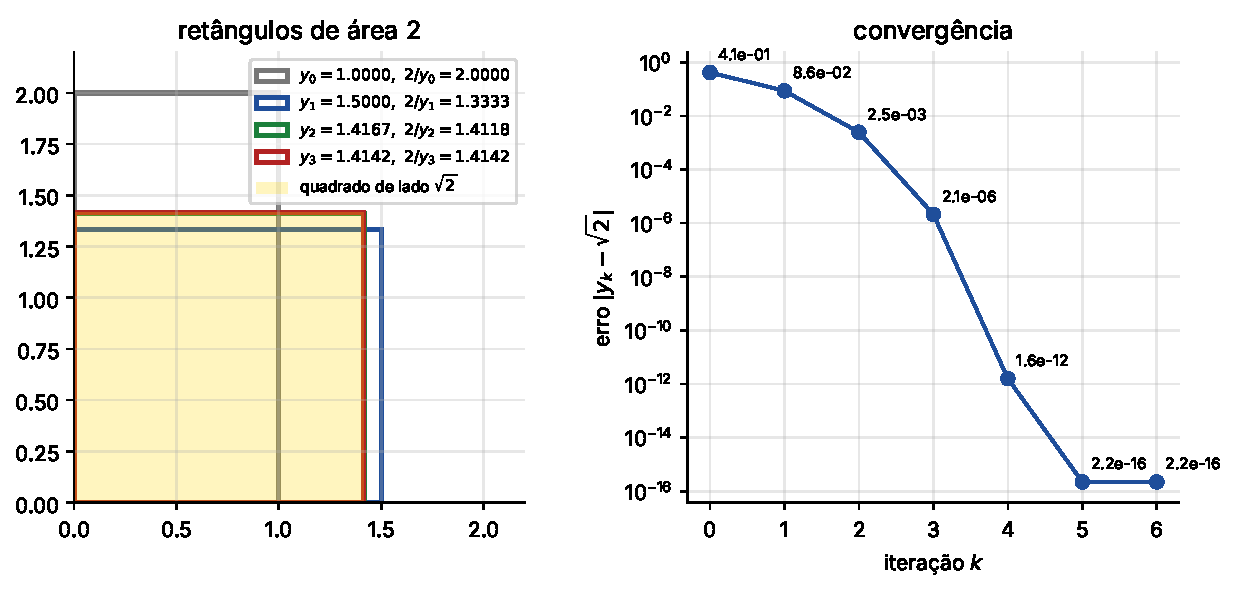
\includegraphics[width=\linewidth]{aula03-babilonico}
\caption{Método babilônico para $\sqrt{2}$, começando com $y_0=1$. À esquerda: os retângulos de área 2 e lados
$y_k$ e $2/y_k$ vão se aproximando de um quadrado. À direita: o erro $|y_k-\sqrt2|$ em escala logarítmica; o número
de casas decimais corretas praticamente dobra a cada passo.}
\label{fig:babilonico}
\end{figure}

\paragraph{Primeira versão.} Seguindo o tutorial do R. Miranda, fazemos um número fixo de repetições:

\begin{entrada}
def minharaizquadrada(x):
    y = 1
    for k in range(1, 10):      # 9 iterações
        y = (y + x/y) / 2
    return y

print(minharaizquadrada(2), math.sqrt(2))
\end{entrada}
\begin{saida}
1.414213562373095 1.4142135623730951
\end{saida}

\paragraph{Acompanhando as iterações.} Vamos imprimir cada aproximação e o seu erro.

\begin{entrada}
x = 2
y = 1.0
for k in range(1, 7):
    y = (y + x/y) / 2
    print(f"k = {k}   y = {y:.16f}   erro = {abs(y - math.sqrt(x)):.2e}")
\end{entrada}
\begin{saida}
k = 1   y = 1.5000000000000000   erro = 8.58e-02
k = 2   y = 1.4166666666666665   erro = 2.45e-03
k = 3   y = 1.4142156862745097   erro = 2.12e-06
k = 4   y = 1.4142135623746899   erro = 1.59e-12
k = 5   y = 1.4142135623730949   erro = 2.22e-16
k = 6   y = 1.4142135623730949   erro = 2.22e-16
\end{saida}

Em apenas 5 passos chegamos ao limite de precisão do \py{float}. Esse método é um caso particular do
\textbf{método de Newton} aplicado a $f(y)=y^2-x$ (que será visto em Cálculo Numérico).

\paragraph{Segunda versão: com critério de parada.} Em vez de um número fixo de passos, paramos quando duas
aproximações consecutivas ficam muito próximas (diferença menor que uma tolerância). Também tratamos os casos
$x<0$ e $x=0$.

\begin{entrada}
def raiz(x, tol=1e-12):
    """Raiz quadrada de x pelo método babilônico."""
    if x < 0:
        print("Erro: x deve ser não negativo")
        return None
    if x == 0:
        return 0.0
    y = x if x > 1 else 1.0          # chute inicial
    passos = 0
    while True:
        novo = (y + x/y) / 2
        passos += 1
        if abs(novo - y) < tol:
            break
        y = novo
    print(f"  ({passos} passos)")
    return novo

for valor in [2, 10, 1e6, 0.0001]:
    r = raiz(valor)
    print(f"raiz({valor}) = {r}   math.sqrt = {math.sqrt(valor)}")
\end{entrada}
\begin{saida}
  (6 passos)
raiz(2) = 1.414213562373095   math.sqrt = 1.4142135623730951
  (7 passos)
raiz(10) = 3.162277660168379   math.sqrt = 3.1622776601683795
  (16 passos)
raiz(1000000.0) = 1000.0   math.sqrt = 1000.0
  (12 passos)
raiz(0.0001) = 0.01   math.sqrt = 0.01
\end{saida}

\begin{desafio}
\begin{enumerate}[label=(\alph*)]
  \item O que acontece se o chute inicial for negativo, por exemplo $y_0=-1$?
  \item Adapte o método para a raiz cúbica, usando $y_{k+1}=\frac{1}{3}\left(2y_k+\frac{x}{y_k^2}\right)$.
  \item (Herão) Calcule $\sqrt{720}$ começando com $y_0=27$ e veja quantos passos são necessários.
\end{enumerate}
\end{desafio}

\begin{professor}
Sugestão: deixar a turma escrever a primeira versão sozinha (10 min) a partir da fórmula no quadro, e só depois
mostrar a tabela de erros. Pergunta para a turma: ``por que o erro para de diminuir em $2{,}22\times10^{-16}$?''
(resposta: é a precisão do \texttt{float}, cerca de 16 algarismos). Para o item (a) do desafio, a sequência
converge para $-\sqrt{x}$.
\end{professor}

% ------------------------------------------------------------
\section{Aplicação: teste de primalidade}
% ------------------------------------------------------------

Na Aula 2 vimos que, para testar se $n$ é primo, basta procurar divisores $d$ com $d\le\sqrt n$. No tutorial do
R. Miranda isso é feito com \py{range(3, int(math.sqrt(n)), 2)}. Vamos testar essa versão:

\begin{entrada}
def checaprimo2(n):
    if n == 2:
        return True
    if n % 2 == 0 or n <= 1:
        return False
    for divisor in range(3, int(math.sqrt(n)), 2):
        if n % divisor == 0:
            return False
    return True

print([n for n in range(2, 60) if checaprimo2(n)])
\end{entrada}
\begin{saida}
[2, 3, 5, 7, 9, 11, 13, 15, 17, 19, 23, 25, 29, 31, 35, 37, 41, 43, 47, 49, 53, 59]
\end{saida}

Há um erro: 9, 15, 25, 35 e 49 aparecem como primos! Como o \py{range} \textbf{não inclui o fim}, o maior
divisor candidato nunca é testado: para $n=15$, \py{int(math.sqrt(15))} vale 3 e \py{range(3, 3, 2)} é vazio;
para $n=49$, o divisor 7 fica de fora. A correção é ir até \py{math.isqrt(n) + 1}:

\begin{entrada}
def eh_primo(n):
    if n == 2:
        return True
    if n % 2 == 0 or n <= 1:
        return False
    for divisor in range(3, math.isqrt(n) + 1, 2):
        if n % divisor == 0:
            return False
    return True

primos = [n for n in range(2, 60) if eh_primo(n)]
print(primos)
print(len([n for n in range(2, 10**5) if eh_primo(n)]), "primos menores que 100000")
\end{entrada}
\begin{saida}
[2, 3, 5, 7, 11, 13, 17, 19, 23, 29, 31, 37, 41, 43, 47, 53, 59]
9592 primos menores que 100000
\end{saida}

\begin{observacao}
O Teorema dos Números Primos diz que a quantidade de primos menores que $N$ é aproximadamente $N/\ln N$. Para
$N=10^5$, \py{1e5 / math.log(1e5)} $\approx 8686$; compare com 9592.
\end{observacao}

% ------------------------------------------------------------
\section{Aplicação: o método da bissecção}
% ------------------------------------------------------------

O Teorema do Valor Intermediário garante: se $f$ é contínua em $[a,b]$ e $f(a)$ e $f(b)$ têm sinais opostos, então
existe $c\in(a,b)$ com $f(c)=0$. O \textbf{método da bissecção} usa isso repetidamente: calcula o ponto médio
$m=\frac{a+b}{2}$ e fica com a metade do intervalo onde a troca de sinal acontece. A cada passo, o
comprimento do intervalo cai pela metade.

\begin{figure}[ht]
\centering
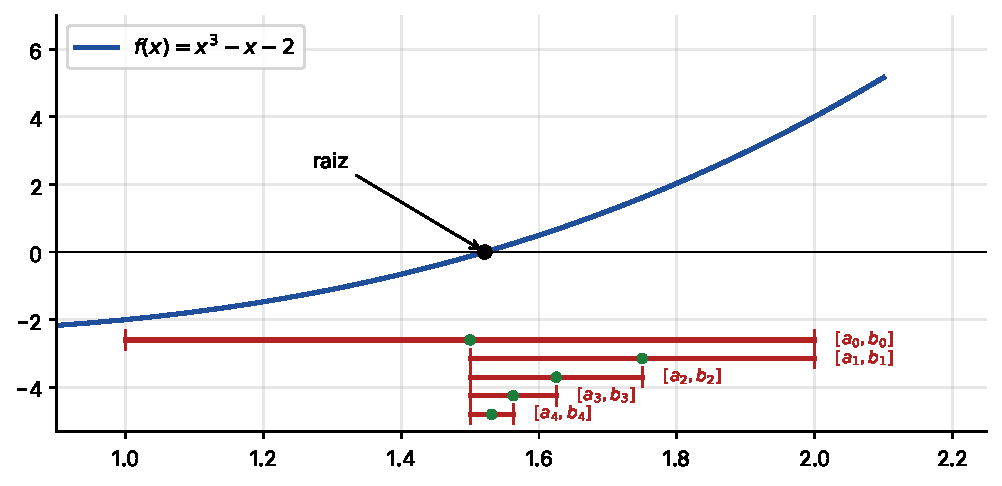
\includegraphics[width=0.9\linewidth]{aula03-bisseccao}
\caption{Bissecção para $f(x)=x^3-x-2$ em $[1,2]$: os intervalos $[a_k,b_k]$ encolhem em torno da raiz.}
\end{figure}

\begin{entrada}
def bisseccao(f, a, b, tol=1e-10):
    if f(a) * f(b) > 0:
        print("f(a) e f(b) têm o mesmo sinal: escolha outro intervalo.")
        return None
    n = 0
    while (b - a) / 2 > tol:
        m = (a + b) / 2
        if f(m) == 0:
            return m
        if f(a) * f(m) < 0:      # a raiz está em [a, m]
            b = m
        else:                    # a raiz está em [m, b]
            a = m
        n += 1
    print(f"  {n} iterações")
    return (a + b) / 2

f = lambda x: x**3 - x - 2
r = bisseccao(f, 1, 2)
print("raiz ~", r, "  f(raiz) =", f(r))

g = lambda x: math.cos(x) - x
print("cos(x) = x  para x ~", bisseccao(g, 0, 1))
\end{entrada}
\begin{saida}
  33 iterações
raiz ~ 1.5213797068572603   f(raiz) = 3.131943593359665e-10
  33 iterações
cos(x) = x  para x ~ 0.7390851332456805
\end{saida}

Como o intervalo é dividido por 2 a cada passo, depois de $n$ passos o erro é no máximo
$\frac{b-a}{2^{n+1}}$. Para garantir erro menor que $10^{-10}$ partindo de $[1,2]$, são necessários
$n\ge \log_2(10^{10})-1\approx 32{,}2$ passos, o que confere com o programa.

% ------------------------------------------------------------
\section{Exercícios}
% ------------------------------------------------------------

\begin{exercicio}[distância e ponto médio]{ex:3-dist}
Escreva uma função \py{distancia(P, Q)} que receba dois pontos do plano como tuplas e devolva a distância entre
eles. Use-a para calcular o perímetro do triângulo de vértices $(0,0)$, $(4,0)$ e $(1,3)$.
\end{exercicio}

\begin{exercicio}[ângulo entre ponteiros]{ex:3-relogio}
Às $h$ horas e $m$ minutos, o ponteiro das horas está a $30h+0{,}5m$ graus da posição das 12h e o dos minutos a
$6m$ graus. Escreva uma função que devolva o menor ângulo entre os ponteiros. Teste com 3h00, 9h45 e 12h30.
\end{exercicio}

\begin{exercicio}[aproximando $e$ e $\pi$]{ex:3-series}
(a) Calcule $\sum_{k=0}^{n}\frac{1}{k!}$ para $n=5,10,15$ e compare com \py{math.e}.
(b) Calcule a série de Leibniz $4\sum_{k=0}^{n}\frac{(-1)^k}{2k+1}$ para $n=10, 1000, 100000$ e compare com
\py{math.pi}. Qual das séries converge mais rápido?
\end{exercicio}

\begin{exercicio}[série de Taylor do seno]{ex:3-seno}
Escreva uma função \py{seno(x, n)} que calcule $\displaystyle\sum_{k=0}^{n}\frac{(-1)^k x^{2k+1}}{(2k+1)!}$ e compare
com \py{math.sin(x)} para $x=1$ e $x=10$, com $n=5$ e $n=20$.
\end{exercicio}

\begin{exercicio}[raiz cúbica]{ex:3-cubica}
Adapte a função \py{raiz} para calcular $\sqrt[3]{x}$ com a iteração $y_{k+1}=\frac{1}{3}\left(2y_k+\frac{x}{y_k^2}\right)$
e compare com \py{math.cbrt}.
\end{exercicio}

\begin{exercicio}[extra: bissecção]{ex:3-bissec}
Use a bissecção para encontrar: (a) a raiz positiva de $x^2-2$ (compare com $\sqrt2$); (b) a solução de
$e^{-x}=x$; (c) a raiz de $x^7+x-1$ em $[0,1]$ (exemplo do tutorial do R. Miranda).
\end{exercicio}
